\documentclass[tikz,border=6pt]{standalone}
\usepackage[T1]{fontenc}
\usepackage[utf8]{inputenc}
\usepackage{pgfplots}
\usepgfplotslibrary{groupplots}
\usetikzlibrary{calc}
\pgfplotsset{compat=1.18}
\begin{document}
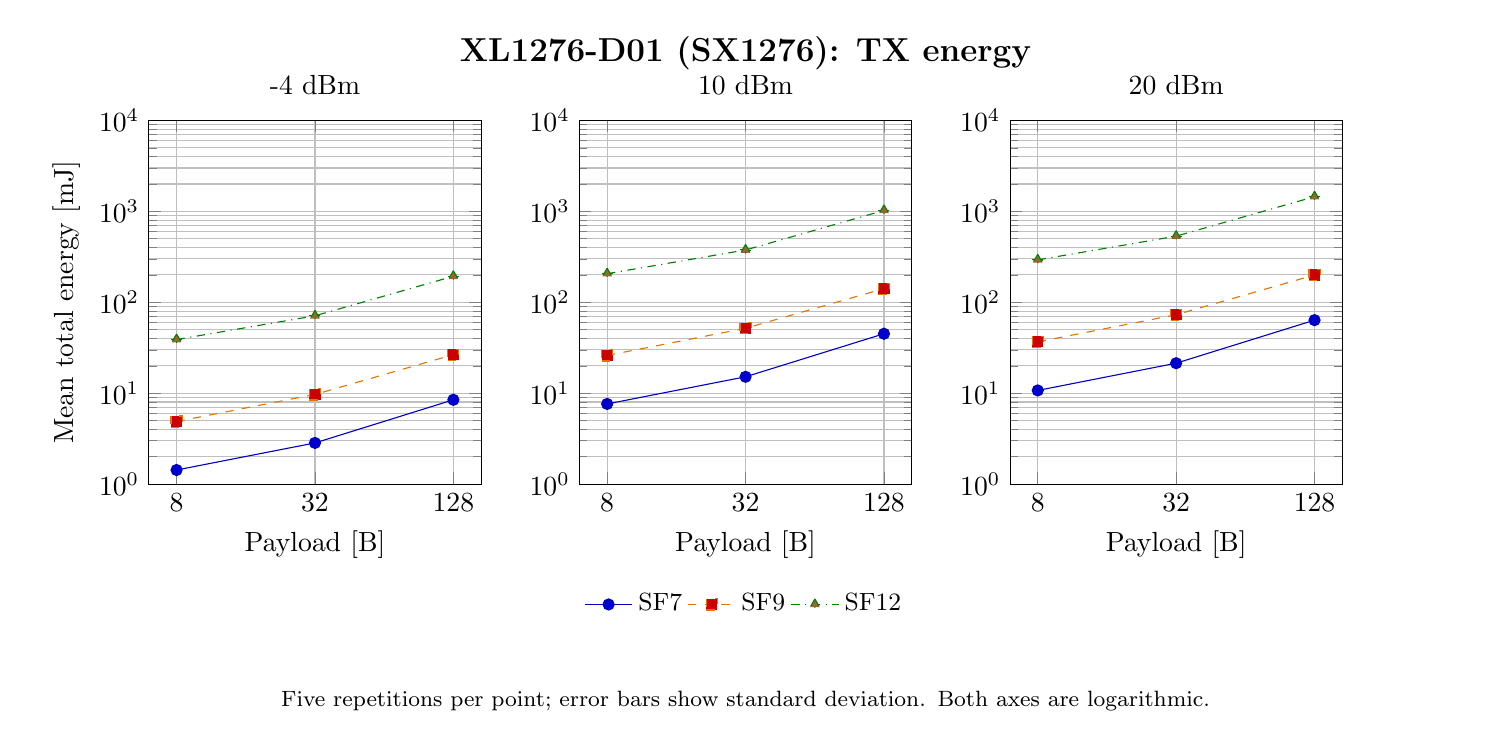
\begin{tikzpicture}
\begin{groupplot}[/pgf/number format/use comma, group style={group size=3 by 1, horizontal sep=1.25cm},
  width=5.8cm,height=6.2cm,xmode=log,log basis x=2,ymode=log,log basis y=10,ymin=1,ymax=10000,
  xtick={8,32,128},xticklabels={8,32,128},grid=both,xlabel={Payload [B]},
  legend style={draw=none,fill=none,font=\small,at={(0.5,-0.27)},anchor=north,legend columns=-1}]
% TX energy
\nextgroupplot[title={-4 dBm},ylabel={Mean total energy [mJ]}]
\addplot+[blue!75!black,solid,mark=*,error bars/.cd,y dir=both,y explicit] coordinates {(8,1.42814239) +- (0,0.00185364218) (32,2.83496753) +- (0,0.00480153101) (128,8.45414023) +- (0,0.0147089527)};
\addplot+[orange!90!black,dashed,mark=square*,error bars/.cd,y dir=both,y explicit] coordinates {(8,4.87190649) +- (0,0.00884155987) (32,9.68344949) +- (0,0.0173648376) (128,26.5091272) +- (0,0.0353878091)};
\addplot+[green!50!black,dashdotted,mark=triangle*,error bars/.cd,y dir=both,y explicit] coordinates {(8,38.8964504) +- (0,0.0252946672) (32,70.9283229) +- (0,0.069671641) (128,193.009991) +- (0,0.203979408)};
\nextgroupplot[title={10 dBm}]
\addplot+[blue!75!black,solid,mark=*,error bars/.cd,y dir=both,y explicit] coordinates {(8,7.60999602) +- (0,0.0424478889) (32,15.1399719) +- (0,0.0891920137) (128,45.0319532) +- (0,0.249228556)};
\addlegendentry{SF7}
\addplot+[orange!90!black,dashed,mark=square*,error bars/.cd,y dir=both,y explicit] coordinates {(8,25.9835918) +- (0,0.127190245) (32,51.7308776) +- (0,0.156903154) (128,141.175698) +- (0,0.637482978)};
\addlegendentry{SF9}
\addplot+[green!50!black,dashdotted,mark=triangle*,error bars/.cd,y dir=both,y explicit] coordinates {(8,206.015716) +- (0,0.681730198) (32,375.763255) +- (0,0.644194208) (128,1023.79057) +- (0,1.61317799)};
\addlegendentry{SF12}
\nextgroupplot[title={20 dBm}]
\addplot+[blue!75!black,solid,mark=*,error bars/.cd,y dir=both,y explicit] coordinates {(8,10.7129874) +- (0,0.0393152079) (32,21.3522876) +- (0,0.0766455207) (128,63.6052744) +- (0,0.195217459)};
\addplot+[orange!90!black,dashed,mark=square*,error bars/.cd,y dir=both,y explicit] coordinates {(8,36.6743408) +- (0,0.101582767) (32,72.9103052) +- (0,0.282399864) (128,199.507278) +- (0,0.520631482)};
\addplot+[green!50!black,dashdotted,mark=triangle*,error bars/.cd,y dir=both,y explicit] coordinates {(8,292.279342) +- (0,0.840966523) (32,533.160977) +- (0,0.602460535) (128,1449.53109) +- (0,1.3158541)};
\end{groupplot}
\node[font=\bfseries\large] at ($(group c2r1.north)+(0,0.85cm)$) {XL1276-D01 (SX1276): TX energy};
\node[font=\footnotesize,align=center,text width=18cm] at ($(group c2r1.south)+(0,-2.75cm)$) {Five repetitions per point; error bars show standard deviation. Both axes are logarithmic.};
\end{tikzpicture}
\end{document}
